\begin{figure}[tbp]
\centering
\includegraphics[width=0.4\textwidth]{figure/cmb_21cm.eps}
\vspace{-0.7cm}
\caption{
    (Top) Constraints on  
    21cm Intensity Mapping and the resolvable modes at $z=1$  
    with the resolution of CHIME and high foregrounds ($R_\parallel=15$ h/Mpc). 
    (Bottom) Constraints on kSZ measurement. Planck noise is estimated at 217 GHz band to avoid tSZ contamination. KSZ effect is calculated for a box of 1.2 Gpc.
}
\label{fig:cmb_21cm}
\end{figure}

Ideally, this velocity reconstruction method should 
retrieve $>90\%$ kSZ signals \citet{Shao11}. 
However, realistic 21cm IM experiments 
can only detect density fluctuations at certain scales, 
as illustrated in Fig.\ref{fig:cmb_21cm}. 
How much cross correlation we could construct is mainly affected 
by three conditions of the experiments:

1. The spacial and velocity resolution of facilities. 

It decides the smallest scale to be observed, 
and the effect could roughly be resembled with a Heaviside Function 
$H(k_\mr{max}-k)$. 
%We choose a realistic $k_\mr{max}$ based on baselines of ongoing experiments 
%\cite{HIRAX,2014SPIE.9145E..22B,2014SPIE.9145E..4VN,2012IJMPS..12..256C,2015ApJ...798...40X}, 
%and an ideal $k_\mr{max}$ based on noise status of Planck Satellite.

2. Foreground noise level:

Foregrounds from Galactic emissions, telescope noises, 
extragalactic radio sources and Radio recombination lines, 
could be three orders brighter than targeted signals\cite{DiMatteo04,Masui13}. 
The process of foreground removal, taking advantage of its low spectral
degrees of freedom \cite{Switzer15}, 
will inevitably contaminates the smooth large scale structure in radial direction.  
To imitate the loss, we apply a high pass filter $W(k_\parallel)=1-e^{-k_\parallel^2R_\parallel^2/2}$. 
%We again test a realistic case \cite{2013ApJ...763L..20M,Switzer13}
%with 
%only half of the signal resolved at $k_\parallel=0.08$ Mpc/h and $0.15$ Mpc/h 
%for redshift 1 and 2 respectively. 
%And a theoretical case \cite{15Shaw} with half of the signal lost 
%at $k_\parallel=0.02$ Mpc/h and $0.04$ Mpc/h for redshift 1 and 2. 
%$R_\parallel=15\ \mr{Mpc}/h$ for $z=1$ and $R_\parallel=8\ \mr{Mpc}/h$ for $z=2$, which gives
%$W_{fs}=0.5$ at
%$k_\parallel=0.08\ \mr{Mpc}/h$ and $0.15\ \mr{Mpc}/h$ respectively. 
%And a good yet still realistic case \cite{15Shaw} with 
%$R_\parallel=60\ \mr{Mpc}/h$ for $z=1$ and $R_\parallel=32\ \mr{Mpc}/h$ for $z=2$, which gives
%$W_{fs}=0.5$ at
%$k_\parallel=0.02\ \mr{Mpc}/h$ and $0.04\ \mr{Mpc}/h$. 
%This is realistic according to the condition of current 21 cm observations 
%\cite{2013ApJ...763L..20M,Switzer13}.

3. The shortest baseline of inteferometers:

Current 21cm IM experiments are all carried on inteferometers. 
To avoid interactions, two beams of a interferometer 
cannot be placed infinitely close. 
The shortest baseline length decides the largest 
angular scale it could probe.  
Structures with angular scale greater than a threshhold of 
$l_\mr{min}$ will be drained out 
in the visibility function 
when cross correlating two beams. 
We again use a Heaviside function to assemble the effect. 
%We do not assume worse cases there, since baselines as short as 20m 
%are already able to filter most of the important modes for velocity reconstruction. 

Therefore, a realistic 21 cm density contrasts will appear as 
\begin{eqnarray}
\label{eq:ns}
    \delta_\mr{IM}(\bm{k})=\delta(\bm{k})H(k_\mr{max}-k)W(k_\parallel)H(l-l_\mr{min}),
\end{eqnarray}

Table.\ref{tab:para} 
lists several representive values for different parameters 
based on previous observations and predictions. 
Fig.\ref{fig:cmb_21cm} 
is a demonstration of density contrasts corresponding to 
$R_\parallel=15$ Mpc/h, $k_\mr{max}=0.6$ h/Mpc 
at $z=1$. 

Directly using $\delta_\mr{IM}$ of any of the parameters 
to reconstruct kSZ signal will 
yields a correlation coeffcient $r<0.2$ 
with observable kSZ signals 
as demonstrated in Fig.\ref{fig:p}.

%With the noise filtered density contrast $\delta_{nf}$, we follow the procedure described in
%section \ref{sec:kszRecon} to generate a mock kSZ signal $\hat \Theta_{nf}$  
%and calculate cross correlation $r_{\Theta\hat\Theta_{nf}}$.

\begin{table}
\begin{tabular}{|m{2cm}|m{1.5cm}|m{1.5cm}|m{1.5cm}|m{1.5cm}|}
    \hline
     & \multicolumn{2}{|c|}{z=1} &\multicolumn{2}{|c|}{z=2}\\
     \hline
     & high foreground &low foreground&high foreground& low foreground\\
     \cline{2-5}
     \footnote{Foreground: smear $k_z\lesssim 0.08,0.02,0.12,0.03$ h/Mpc respectively. Parameters based on \cite{2013ApJ...763L..20M,Switzer13,15Shaw}}
     $R_\parallel$ Mpc/h
      & 15 & 60 & 10 & 40 \\
     \hline
     & CHIME & HIRAX & CHIME &HIRAX\\
     \cline{2-5}
     \footnote{Small scale noises: based on CHIME\cite{2014CHIME} and HIRAX\cite{HIRAX} 
     with 100 m and 200 m longest baseline respectively.}
     $k_\mr{max}$ h/Mpc 
     & 0.6 & 1.2 & 0.4 & 0.8 \\
     \hline
     \footnote{Spatial loss of inteferomenter: assuming shortest baseline of 20 m.}
     $\ell_\mr{min}$
     & \multicolumn{4}{|c|}{300} \\
     \hline
\end{tabular}
     \caption{Parameter of different noise filtering.}
     \label{tab:para}
\end{table}
